% !TEX root =  main.tex
\chapter{Approach}
\label{chap:approach}
\pagestyle{plain}

This chapter describes the proposed framework for training learned cardinality estimators using LLM-generated workloads and active learning. First, the overall system architecture and workflow are presented. The chapter then discusses key pipeline properties including modularity, schema independence, reliability, and reproducibility.

Effective training of a learned cardinality estimator requires balancing two conflicting requirements: the availability of a large, diverse set of labeled queries and the practical constraints associated with obtaining such labels. Each label demands executing a query on a live database, which is slow and expensive. The proposed framework addresses this challenge by integrating query generation, labeling, feature extraction, active learning, and evaluation into a unified workflow.

\section{System Architecture}

The system integrates four stages into a largely automated workflow, with environment-specific setup (database access, model runtime, and schema artifacts) handled before execution. Figure~\ref{fig:Pipeline} illustrates how data flows from the database schema to the trained estimator and evaluation outputs.

\begin{figure}[tbp]
\centering
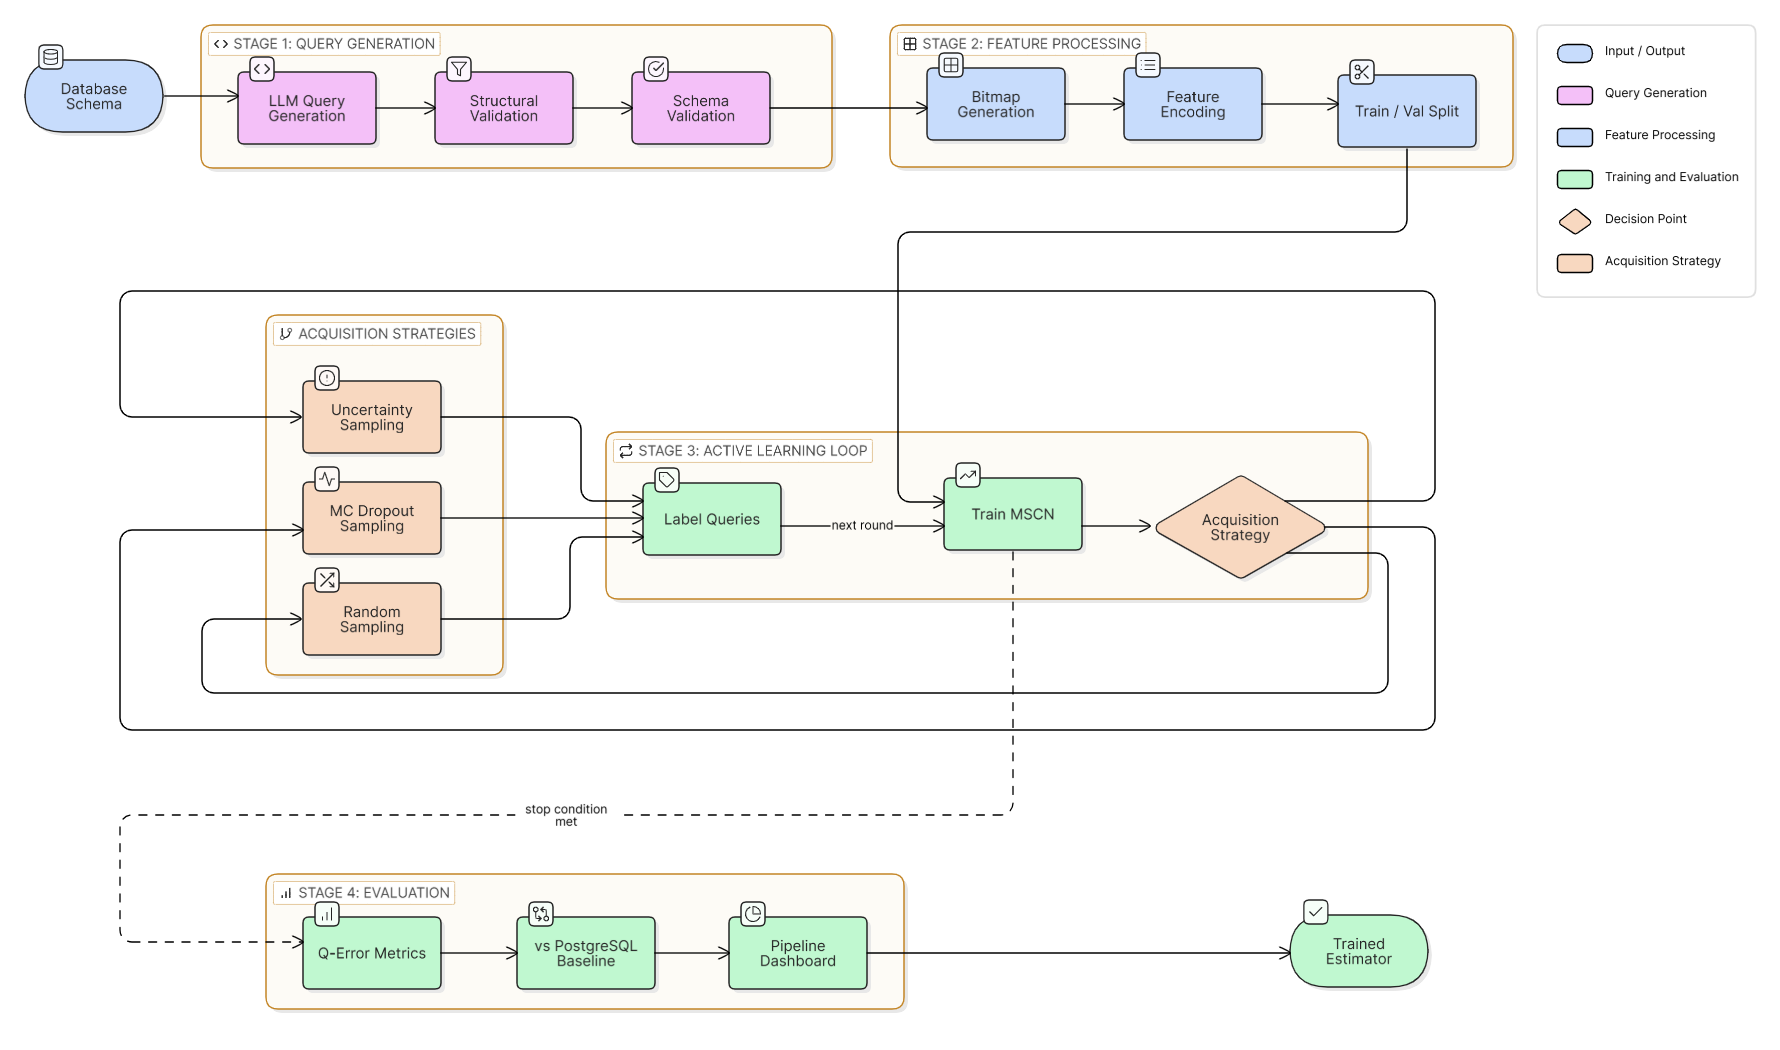
\includegraphics[width=\textwidth]{Report/graphs/pipeline.png}
\caption{Overview of the Proposed End-to-End Pipeline}
\label{fig:Pipeline}
\end{figure}

The pipeline begins with query generation. The database schema and column statistics are provided to a large language model, which generates batches of \texttt{SELECT COUNT(*)} queries representing diverse analytical workloads. The generated queries contain varying join structures, predicate combinations, and selectivity patterns. For environments where LLM-based generation is impractical, the framework also supports a deterministic synthetic query generator. Chapter~\ref{chap:query_generation} explains the prompt design, diversity mechanisms, and the comprehensive four-layer validation process used to detect malformed or unsupported queries before they are executed.

Validated queries are then labeled by executing them against PostgreSQL to obtain ground-truth cardinalities. For each query, the framework reconstructs a corresponding \texttt{SELECT COUNT(*)} statement and records the returned row count. Query execution represents the most computationally expensive stage of the pipeline, particularly for complex join queries and large workloads. This execution cost motivates the integration of active learning to reduce the number of queries requiring labeling.

Before training, each query is converted into a fixed-size tensor representation for neural processing. Each query is decomposed into tables, predicates, and joins. Individual elements are encoded using one-hot vectors and bitmap representations indicating which sampled rows satisfy the query predicates. These bitmaps capture data distributions together with query structure. The complete encoding process and MSCN architecture are described in Chapter~\ref{chap:training_approach}.

The active learning loop integrates model training, query selection, and labeling into a single iterative workflow. Training begins with a small randomly labeled seed set used to initialize the MSCN model. After the initial training phase, the model evaluates the remaining unlabeled queries, and the acquisition function ranks candidate samples according to the selected acquisition strategy. The highest-ranked queries are then executed to obtain ground-truth labels and incorporated into the training set before the model is retrained.

The framework implemented in this work supports three acquisition strategies: random sampling and MC Dropout variance-based sampling. These strategies represent different trade-offs between acquisition overhead and label efficiency. These strategies represent different trade-offs between computational overhead and labeling efficiency. A detailed discussion of the active learning framework, acquisition functions, and experimental configuration is presented in Chapter~\ref{chap:active_learning}.


\section{Pipeline Properties}

Several properties distinguish the proposed framework from earlier approaches to learned cardinality estimation. The pipeline is designed to operate across relational schemas containing defined foreign-key relationships. Given table definitions, column types, and join relationships, the framework automatically generates queries, validates them, extracts features, and trains the estimator without requiring workload-specific query engineering or benchmark-specific preprocessing. Consequently, the same implementation can be adapted to different database schemas without modifications to the overall pipeline structure. This portability is important because learned cardinality estimators must be retrained efficiently as schemas and workloads evolve over time.

Each stage of the pipeline is implemented as an independent component with clearly separated responsibilities. For example, the query generation module can be configured to use different large language models or alternative generation mechanisms, such as rule-based or template-based approaches, without requiring modifications to the remaining stages of the pipeline. Similarly, both the acquisition strategy used during active learning and the neural network architecture employed for estimation can be replaced independently. This modular design supports controlled experimentation by allowing individual components to be evaluated in isolation.

The framework additionally incorporates mechanisms to ensure reliable execution during large-scale processing. Queries that exceed the execution time limit are retried using a back-off strategy, while queries that continue to fail after all retry attempts are discarded from the final labeled workload. Rollback and cleanup procedures ensure that failed executions do not affect subsequent queries. As a result, the system can process large workloads with minimal manual intervention while preserving the quality of collected supervision signals.

The framework also incorporates several mechanisms to improve experimental reproducibility. Random seeds are consistently applied across Python, NumPy, and PyTorch in order to reduce nondeterministic behavior during training. Furthermore, all hyperparameters are logged alongside experimental outputs, and timestamped result directories prevent runs from accidentally overwriting previous results.